\documentclass[12pt]{ctexart} 
\usepackage{array}
\usepackage{geometry}  
\usepackage{graphicx}  
\usepackage{amsmath, amssymb}  
\usepackage{booktabs}  
\usepackage{enumerate} 
\usepackage{verbatim}
\usepackage{url}
\usepackage{fancyhdr}  % 引入 fancyhdr 包
\pagestyle{fancy}  % 使用 fancy 页眉页脚样式
\fancyhf{}  % 清空默认的页眉页脚
\fancyfoot[C]{\thepage}  % 在底部中央显示页码
\renewcommand{\headrulewidth}{0pt}  % 去掉页眉的横线
%\pagestyle{empty}  % 去掉页眉和页脚的页码
% 页面设置  
\geometry{a4paper, margin=2.5cm}  
\setlength{\parindent}{2em} % 2em 相当于两个字符的宽度

%\title{基于收益最大化的种植策略探究}  
%\author{张文瑞、陈名湛、王晨屹}  
%\date{\today}  


\begin{document}
	\section*{CT}
	
	\begin{center}
		\Large\textbf{摘要}
	\end{center}
	
	CT 技术在当代社会已广泛应用在临床医学、工业工程等领域。在本题中首先通过建立离散模型并对其简化从而对 CT 仪器参数进行了标定;建立平行束滤波反投影重建模型,通过 Radon 变换及 R-L 滤波器解决了成像问题,并通过对平行束滤波反投影重建模型进行优化,使模型具有降噪能力,从而得到了更精确符合实际的图形与吸收率值。
	
	\noindent {\textbf{关键词:}}
	
	
	\newpage
	
	\section{问题重述}
	
	CT可以在不破坏样品的情况下,利用样品对射线能量的吸收特性对生物组织和工
	程材料的样品进行断层成像,由此获取样品内部的结构信息。本题X射线的发射器和探
	测器的相对位置固定不变,整个发射-接收系统绕位于正方形托盘下方某处旋转中心逆
	时针旋转180次。对每一个X射线方向,发射接收装置装有512个等距单元探测器,用
	于测量位置固定不动的二维待测介质吸收衰减后的射线能量,并且通过增益等处理方式
	得到180组接收信息。然而由于存在系统误差,所以需要对安装好的CT系统进行参数
	标定,通过已知模板对CT系统的参数进行标定,并根据标定的参数对未知结构的样品
	进行成像。
	
	具体问题重述如下:
	
	\noindent
	(1) 在正方形托盘上放置两个均匀固体介质组成标定模板,模板的几何信息如图2给出,
	相应的数据文件见附件1,其中每一点的数据值反映了该点的吸收强度“吸收率”。
	应用于模板的接收信息见附件2。问题一要求根据模板及其接收信息对 \textbf{CT 系统} 进行参数标定,
	确定出此 \textbf{CT 系统} 实际的旋转中心在正方形托盘中的位置、探测器单元间距离以及该 \textbf{CT 系统} 使用的 \textbf{X 射线} 的180个方向。
	
	\noindent
	(2) 利用问题一所标定的 \textbf{CT 系统} 相关参数以及所建立模型,使用附件3所给未知介质的接收信息,
	确定出该未知介质在正方形托盘中的位置、几何形状以及吸收率等信息。另外利用附件4中数据给出图3中所给10个位置处的吸收率。
	
	\noindent
	(3) 附件5为利用该 \textbf{CT 系统} 得到的另一未知介质的接收信息。同样利用问题1中的标定参数与模型,
	给出未知介质的系列相关信息并给出图3中10个位置处的吸收率。

	\noindent
	(4) 对问题1中参数标定的精度以及稳定性进行分析,并在此基础上建立新模型,建立对应的标定模型,
	以改进标定精度和稳定性,并说明理由。
	
	\begin{figure}[htbp]
		\centering
		\begin{minipage}[t]{0.32\textwidth}
			\centering
			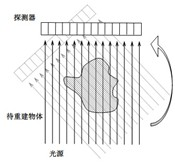
\includegraphics[width=\textwidth]{CT系统示意图.jpg}
			\caption{CT系统示意图}
		\end{minipage}
		\begin{minipage}[t]{0.32\textwidth}
			\centering
			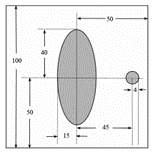
\includegraphics[width=\textwidth]{模板示意图.png}
			\caption{模板示意图}
		\end{minipage}
		\begin{minipage}[t]{0.32\textwidth}
			\centering
			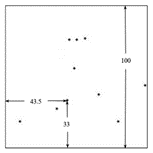
\includegraphics[width=\textwidth]{十个位置示意图.png}
			\caption{十个位置示意图}
		\end{minipage}
	\end{figure}
	
	%怎么列表????
	
	
	\section{问题分析}
	
	\section{模型假设}
	
	\section{符号说明}
	
	\section{问题一求解}
	\subsection{理论基础}
	
	由所阅读的文献,CT 机通常对衰减系数公式做如下处理:
	\begin{equation}
		P = \ln \frac{I_0}{I} = \mu L
	\end{equation}
	
	问题中,使用的 CT 系统的原理是使用 X 射线照射在样品上物体吸收部分射线的能量,使得射线强度产生衰减,射线的衰减呈指数变化。那么对于长度为$l$的均匀同质物体,吸收率为$\rho$,则探测器上对应位置得到的接收信息 D 应满足:
	\begin{equation}
		D = f(\rho l)
		\label{D}
	\end{equation}
	
	\subsection{数据分析}
	
	通过分析附件一和附件二,我们得到了如下信息:
	\begin{figure}[htbp]
		\centering
		\begin{minipage}[t]{0.45\textwidth}
			\centering
			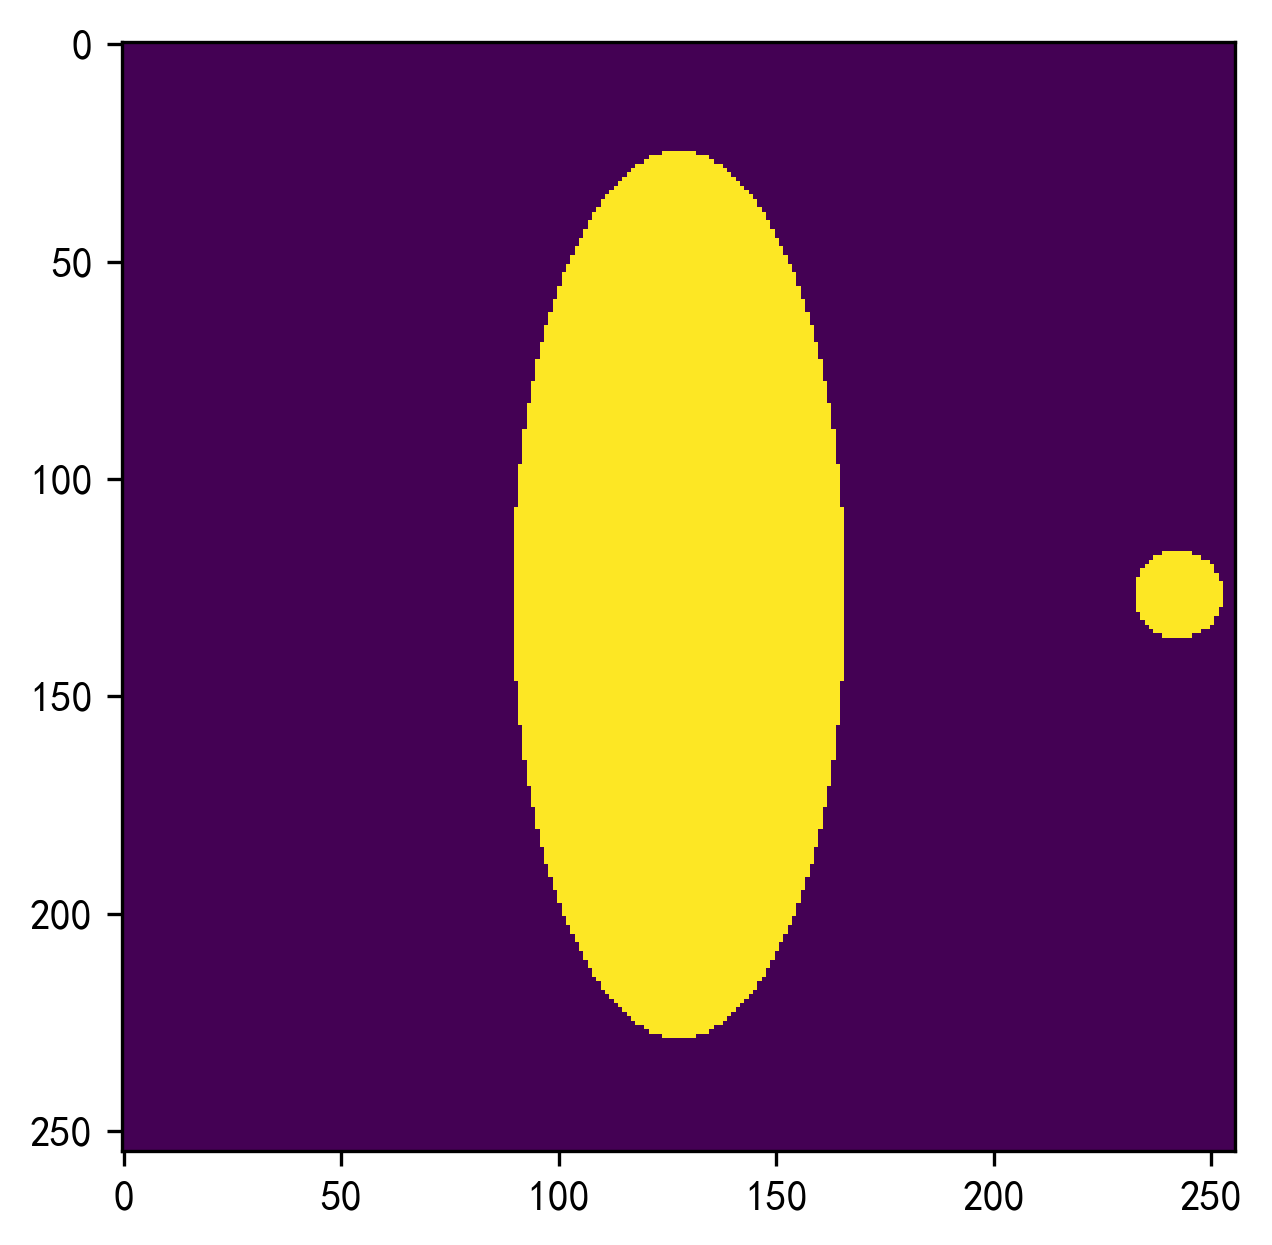
\includegraphics[width=\textwidth]{附件1信息.png}
			\caption{附件1信息}
			\label{附件1}
		\end{minipage}
		\begin{minipage}[t]{0.45\textwidth}
			\centering
			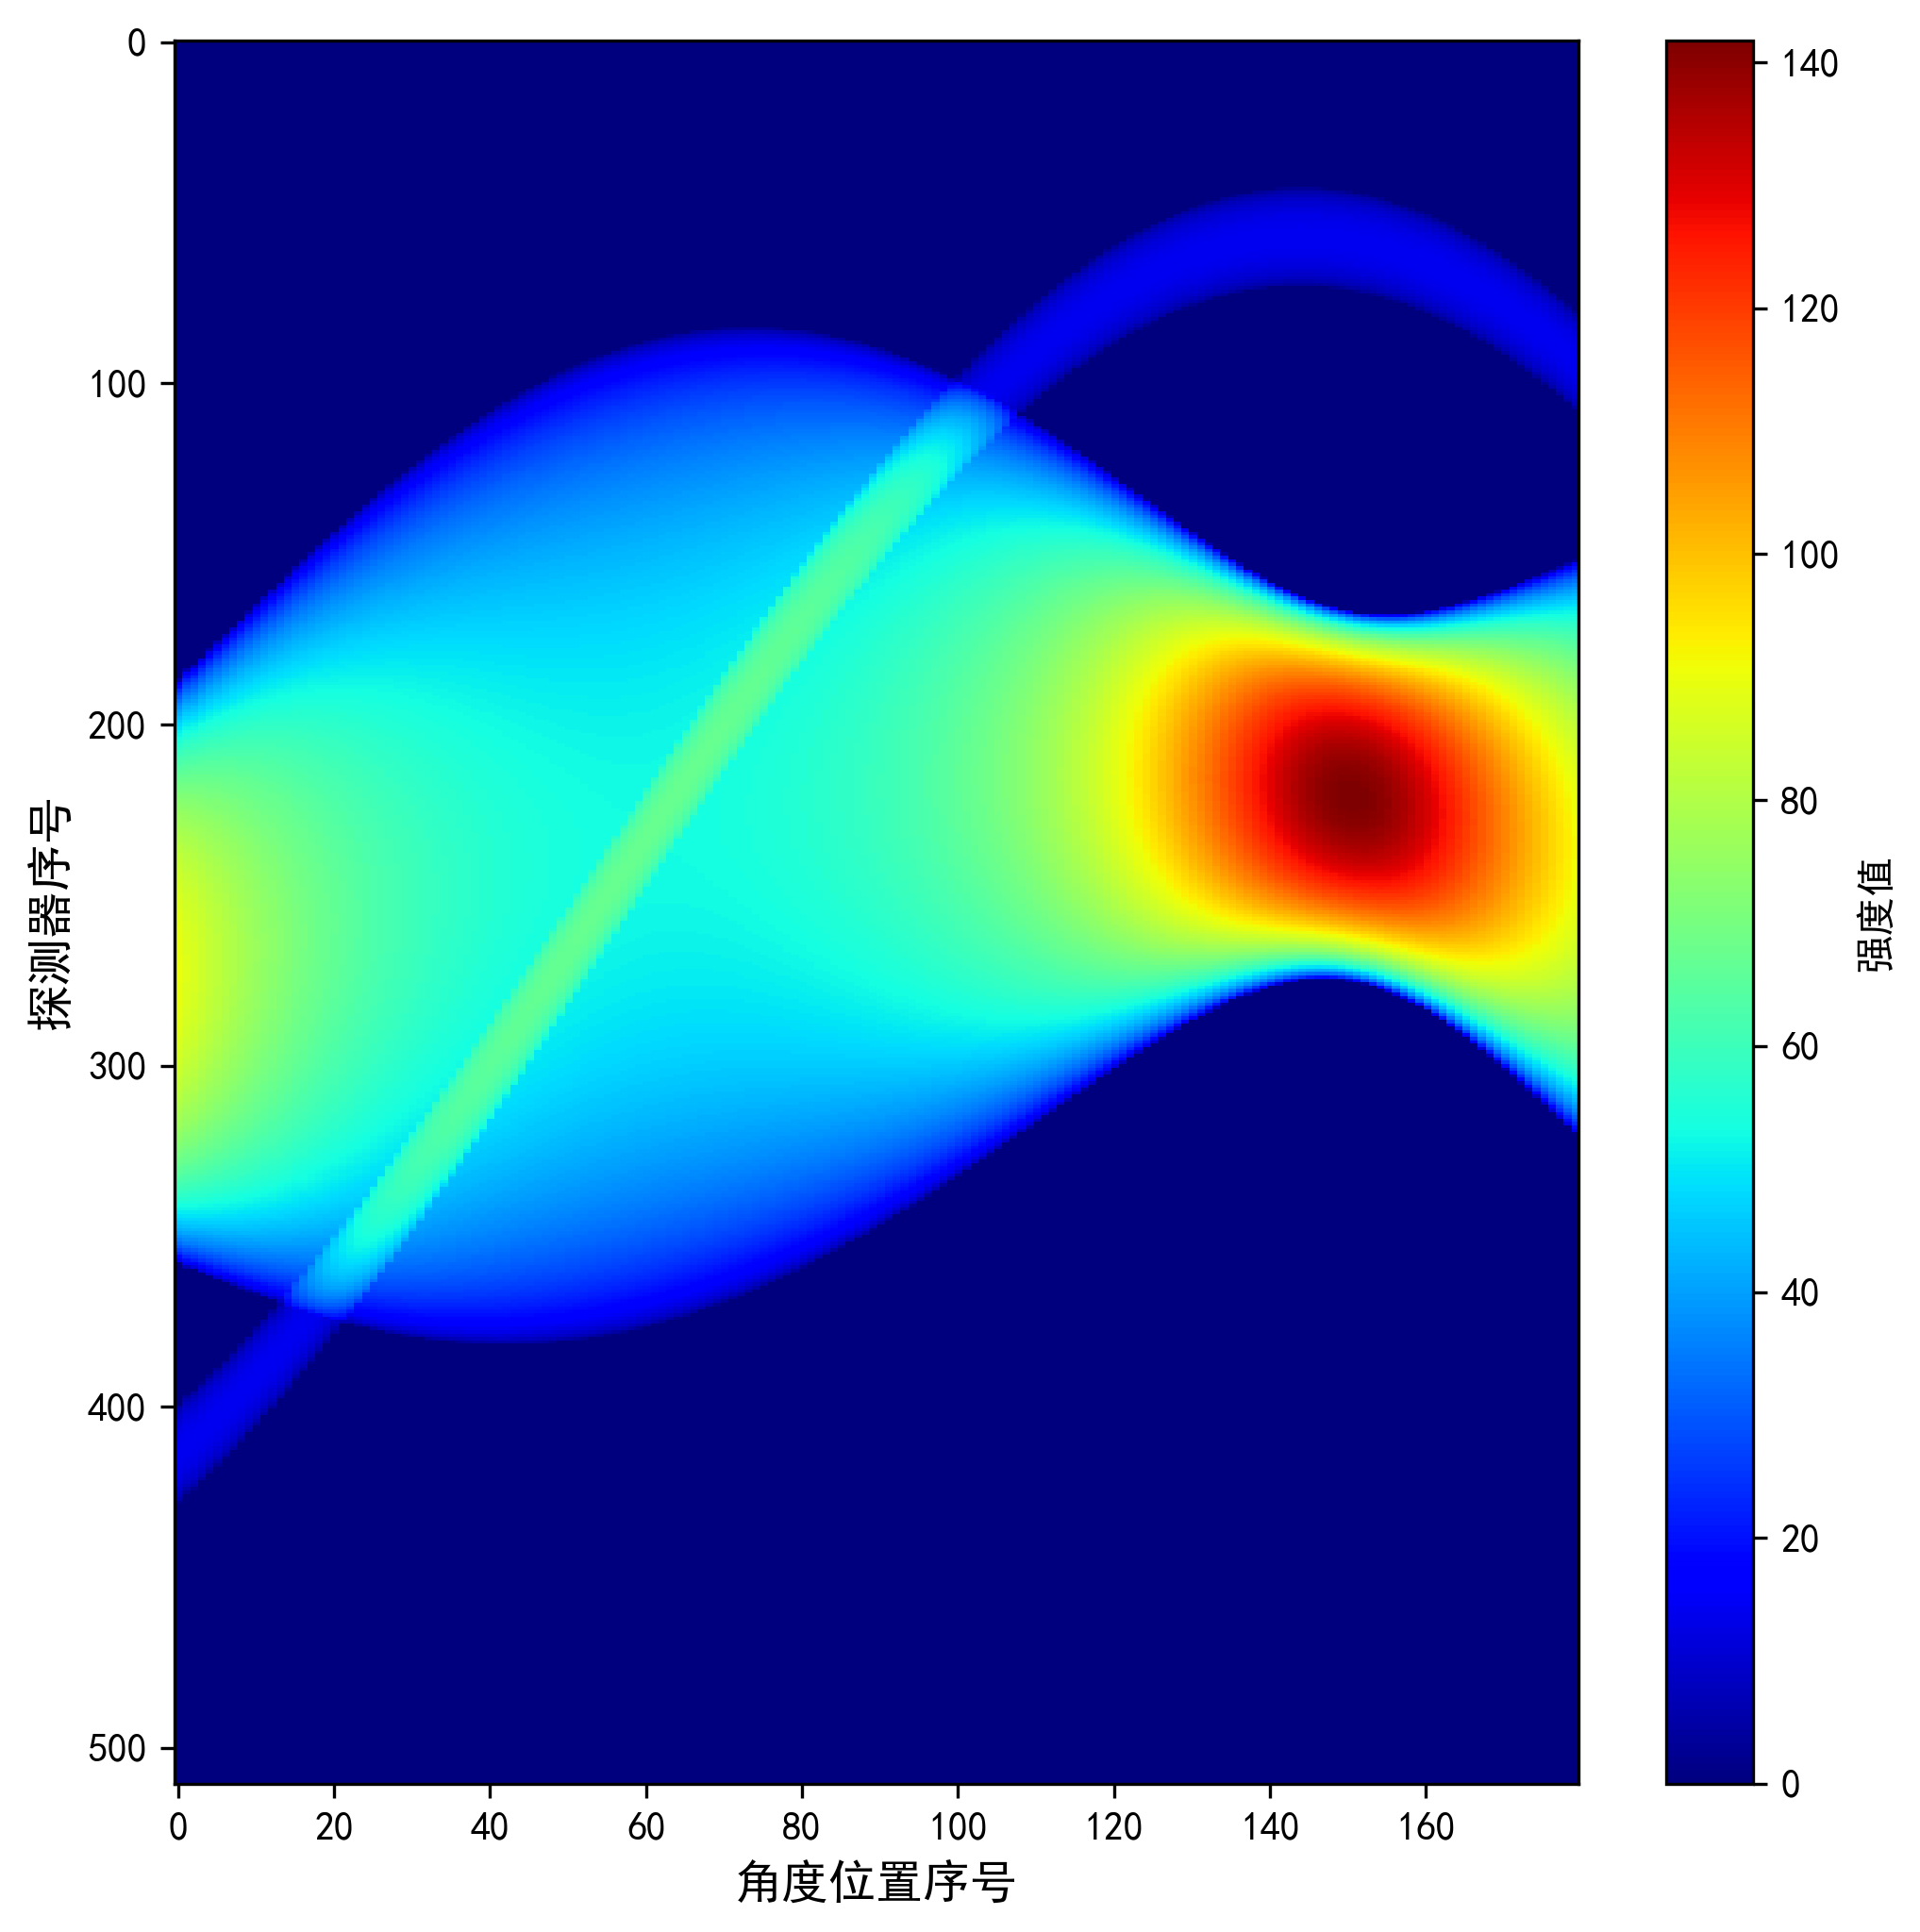
\includegraphics[width=\textwidth]{附件2信息.png}
			\caption{附件2信息}
			\label{附件2}
		\end{minipage}
	\end{figure}
	
	根据图\ref{附件2},我们可以明显地看出窄条为圆形模板的投影,而另一部分是椭圆形模板的投影,并且二者有重叠部分。二者重叠部分为X射线同时穿过椭圆和圆形模板,而为0的地方则表示X射线经过空气直接打到单元探测器上。
	
	\subsection{理论公式}
	
	在此问题中,介质为均匀介质且吸收率为$1$,根据公式\ref{D},此时探测器获得的数值即与穿过的长度有关。在这一问题中,我们转换成某一方向的直线穿过标定模板的长度求解。
	
	我们假设椭圆中心为坐标原点,椭圆中心与圆中心连线为X轴,过坐标原点垂直于 x 轴方向为 y 轴,建立平面直角坐标系。旋转中心假设为$R(x_0,y_0)$,标定模板椭圆和圆的方程分别为:
	\begin{equation*}
		\frac{x^2}{m^2} + \frac{y^2}{n^2} = 1,m=15,n=40 ; (x - 45)^2 + y^2 = 4^2
	\end{equation*}
	
	由于题目中X射线会进行旋转,故我们假设长度为$d$的射线旋转角度为$\theta$,则射线长度公式为
	\begin{equation*}
		x\cos\theta + y\sin\theta = d
	\end{equation*}
	
	与椭圆方程进行联立,可求得该射线与椭圆相交弦长长度:
	\begin{equation*}
		p = \frac{2mn \sqrt{r^2 - d^2}}{r^2},\text{这里 } r^2 = m^2 \cos^2 \theta + n^2 \sin^2 \theta
	\end{equation*}
	
	对于圆上的部分,设圆心坐标为$(G, 0)$,圆半径为$r_0$,其中$G = 45,r_0 = 4$,那么容易求出其弦长表达式为:
	\begin{equation*}
		p_1 = 2 \sqrt{r_0^2 - (G \cos \theta - d)^2}
	\end{equation*}
	同时,由于在整个旋转过程中,直线与椭圆或圆不一定有交点,那么这种情况下,我们对整个角度范围进行整合,可以得到总的投影长度为:
	\begin{equation*}
		p_t = \frac{2mn \sqrt{\max(0, m^2 \cos^2 \theta + n^2 \sin^2 \theta - d^2)}}{m^2 \cos^2 \theta + n^2 \sin^2 \theta}
		+ 2 \sqrt{\max(0, r_0^2 - (G \cos \theta - d)^2)}
	\end{equation*}
	
	考虑到实际情况中,探测器的中心与坐标原点有一定的偏移,那么在上式的基础上,我们
	需要对投影长度进行修正。
	
	易证,在探测器能探测到物体的前提下,沿垂直于探测器方向的探测器位置变化对投
	影长度没有影响。即在探测器位置发生变化时,只需要考虑沿探测器方向的位置变化。
	
	那么对于旋转中心坐标 $R(x_0, y_0)$,探测器中心与旋转中心在探测器平面上的投影的有向距离$d_0$,对于探测器上一条射线,其与探测器中心的距离为$d$,那么容易求出,该点与坐标原点在探测器上的投影的距离$d'$的值为:
	\begin{equation*}
		d' = x_0 \cos \theta + y_0 \sin \theta + d_0 + d
	\end{equation*}
	
	\section{问题二求解}
	\subsection{定义目标函数}
	\subsection{构造价格的概率分布模型}
	\subsubsection{GBM描述价格的微分方程}
	\subsubsection{对数收益形式}
	\subsubsection{模拟收益生成路径}
	\subsubsection{计算风险度量}
	\subsection{条件约束}
	\subsubsection{种植面积总和约束}
	\subsubsection{非负性约束}
	\subsubsection{地块类型与用途约束}
	\subsubsection{可持续性发展约束}
	\subsubsection{风险控制约束}
	\subsection{鲁棒优化模型求解}
	\subsubsection{定义决策变量}
	\subsubsection{确定目标函数}
	\subsubsection{输出结果}
	
	\newpage
	\section{问题三求解}
	\subsection{预期销售量、亩产量和种植成本的相关性分析}
	\subsection{建立交叉弹性矩阵}
	\subsection{条件约束}
	\subsubsection{种植面积总和约束}
	\subsubsection{非负性约束}
	\subsubsection{地块类型与用途约束}
	\subsubsection{可持续性发展约束}
	\subsubsection{风险控制约束}
	\subsubsection{交叉弹性约束}
	\subsection{适应度函数}
	\subsection{模型求解}
	\subsubsection{数据输入}
	\subsubsection{定义聚类中心}
	\subsubsection{初始化}
	\subsubsection{簇分配}
	\subsubsection{质心更新}
	\subsubsection{目标函数}
	\subsubsection{算法终止判定}
	\subsubsection{结果输出}
	\subsection{比较分析}
	
	\newpage
	\section{模型的检验}
	\subsection*{1. 残差P-P图}
	\subsection*{2. 单样本K-S检验}
	\subsection*{3. 灵敏度分析}
	
	\section{模型的评价与改进}
	\subsection{模型的优点}
	\subsection{模型的缺点}
	\subsection{模型的改进}
	
	\newpage
	\begin{thebibliography}{9}
		
	\end{thebibliography}
	
	\newpage
	\section*{附录}
	\subsection*{附录1 支撑材料}
	
	\newpage
	\section{问题一第一小问代码}
	
	\section{问题一第二小问代码}
	
	\section{问题二代码}
	
	\section{问题三代码}
	
	
	
\end{document}